
\section{System Model}
\label{sec:model}

To characterize coordination avoidance, we first present a system
model. We begin with an informal overview. In our model, transactions
operate over independent (logical) ``snapshots'' of database
state. Transaction writes are applied at one or more snapshots
initially when the transaction commits and then are integrated into
other snapshots asynchronously via a ``merge'' operator that
incorporates those changes into the snapshot's state. Given a set of
invariants describing valid database states, as
Table~\ref{table:requirements} outlines, we seek to understand when it
is possible to ensure invariants are always satisfied (global
validity) while guaranteeing a response (transactional availability)
and the existence of a common state (convergence), all without
communication during transaction execution
(coordination-freedom). This model need not directly correspond
to a given implementation (e.g., see the database architecture in
Section~\ref{sec:evaluation})---rather, it serves as a useful
abstraction.  The remainder of this section
further defines these concepts; readers more interested in their
application should proceed to Section~\ref{sec:bcc-theory}. We provide
greater detail and additional discussion in~\cite{ca-extended}.

\begin{table}[t]
\begin{center}
\small
\begin{tabular}{|l|r|}
  \hline\textbf{Property} & \textbf{Effect}  \\\hline
  Global validity & Invariants hold over committed states  \\
  Transactional availability & Non-trivial response guaranteed \\
  Convergence & Updates are reflected in shared state \\
  Coordination-freedom & No synchronous coordination\\\hline
\end{tabular}
\end{center}\vspace{-1em}
\caption{Key properties of the system model and their effects.}
\label{table:requirements}
\end{table}

\minihead{Databases} We represent a state of the shared database as a
set $D$ of unique \textit{versions} of data items located on an arbitrary set of
database servers, and each version is located on at least one
server. We use ${\cal D}$ to denote the set of possible database
states---that is, the set of sets of versions. The database is
initially populated by an initial state $D_0$ (typically but not
necessarily empty).

\minihead{Transactions, Replicas, and Merging} Application clients
submit requests to the database in the form of transactions, or
ordered groups of operations on data items that should be executed
together. Each transaction operates on a logical \textit{replica}, or
set of versions of the items mentioned in the transaction. At the
beginning of the transaction, the replica contains a subset of the
database state and is formed from all of the versions of the relevant
items that can be found at one or more physical servers that are
contacted during transaction execution. As the transaction executes,
it may add versions (of items in its writeset) to its replica. Thus,
we define a transaction $T$ as a transformation on a replica: $T:
{\cal D}\rightarrow {\cal D}$. We treat transactions as opaque
transformations that can contain writes (which add new versions to the
replica's set of versions) or reads (which return a specific set of
versions from the replica). (Later, we will discuss transactions
operating on data types such as counters.)

Upon completion, each transaction can \textit{commit}, signaling
success, or \textit{abort}, signaling failure. Upon commit, the
replica state is subsequently \textit{merged} ($\sqcup$:${\cal D}
\times {\cal D} \rightarrow {\cal D}$) into the set of versions at
least one server. We require that the merged effects of a committed
transaction will eventually become visible to other transactions that
later begin execution on the same server.\footnote{This implicitly
  disallows servers from always returning the initial database state
  when they have newer writes on hand. This is a relatively pragmatic
  assumption but also simplifies our later reasoning about admissible
  executions. This assumption could possibly be relaxed by adapting
  Newman's lemma~\cite{obs-confluence}, but we do not consider the
  possibility here.}  Over time, effects propagate to other servers,
again through the use of the merge operator.  Though not strictly
necessary, we assume this merge operator is commutative, associative,
and idempotent~\cite{calm,crdt} and that, for all states $D_i$, $D_0
\sqcup D_i = D_i$.  In our initial model, we define
merge as set union of the versions contained at different servers.
(Section~\ref{sec:bcc-practice} discusses additional implementations.)
For example, if server $R_x = \{v\}$ and $R_y = \{w\}$, then $R_x
\sqcup R_y = \{v, w\}$.

In effect, each transaction can modify its replica state without
modifying any other concurrently executing transactions' replica
state. Replicas therefore provide transactions with partial
``snapshot'' views of global state (that we will use to simulate
concurrent executions, similar to revision
diagrams~\cite{ec-txns}). Importantly, two transactions' replicas do
not necessarily correspond to two physically separate servers; rather,
a replica is simply a partial ``view'' over the global state of the
database system. For now, we assume transactions are known in advance
(see also~\rsection{8}).

\minihead{Invariants} To determine whether a database state is valid
according to application correctness criteria, we use
\textit{invariants}, or predicates over replica state: $I: {\cal D}
\rightarrow \{true, false\}$~\cite{eswaran-consistency}.  In our
payroll example, we could specify an invariant that only one user in a
database has a given ID. This invariant---as well as almost all
invariants we consider---is naturally expressed as a part of the
database schema (e.g., via DDL); however, our approach allows us to
reason about invariants even if they are known to the developer but
not declared to the system. Invariants directly capture the notion of
ACID Consistency~\cite{bernstein-book,gray-virtues}, and we say that a
database state is \textit{valid} under an invariant $I$ (or $I$-valid)
if it satisfies the predicate:

\begin{definition}
A replica state $R \in {\cal D}$ is \textit{$I$-valid} iff $I(R) = true$.
\end{definition}

We require that $D_0$ be valid under
invariants. Section~\ref{sec:theory-discussion} provides additional discussion
regarding our use of invariants.

% Unlike more general forms of axiomatic logic (e.g., Hoare-style triples~\cite{decomp-semantics,isolation-semantics}), we require only one set of invariants per application.

\minihead{Availability} To ensure each transaction receives a
non-trivial response,
we adopt the following definition of
\textit{availability}~\cite{hat-vldb}:

\begin{definition} 
  A system provides \textit{transactionally available} execution iff,
  whenever a client executing a transaction $T$ can access servers
  containing one or more versions of each item in $T$, then $T$
  eventually commits or aborts itself either due to an \textit{abort}
  operation in $T$ or if committing the transaction would violate a
  declared invariant over $T$'s replica state. $T$ will commit in all
  other cases.
\end{definition}

Under the above definition, a transaction can only abort if it
explicitly chooses to abort itself or if committing would violate
invariants over the transaction's replica state.\footnote{This basic
  definition precludes fault tolerance (i.e., durability) guarantees
  beyond a single server failure~\cite{hat-vldb}. We can relax this
  requirement and allow communication with a fixed number of servers
  (e.g., $F+1$ servers for $F$-fault tolerance; $F$ is often
  small~\cite{dynamo}) without affecting our results. This does not
  affect scalability because, as more replicas are added, the
  communication overhead required for durability remains constant.}


\begin{figure}
\begin{center}
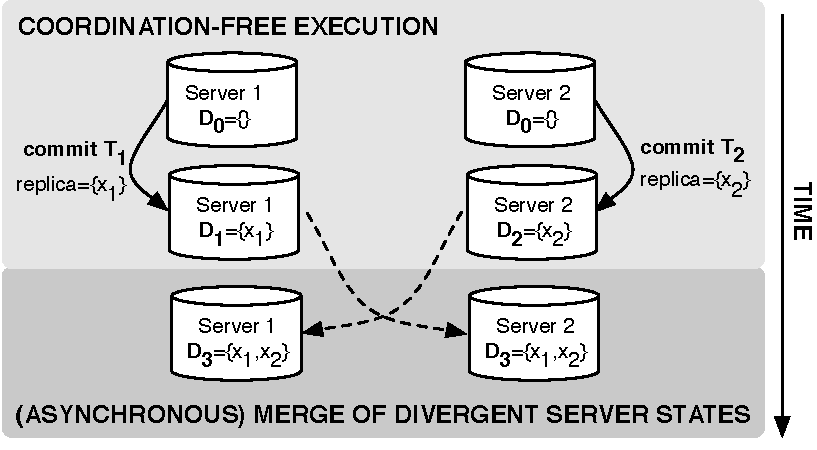
\includegraphics[width=.85\columnwidth]{figs/replicas.pdf}
\end{center}\vspace{-2em}
\caption{An example coordination-free execution of two transactions,
  $T_1$ and $T_2$, on two servers. Each transaction writes to its
  local replica, then, after commit, the servers asynchronously
  exchange state and converge to a common state ($D_3$).}
\label{fig:replicas}
\end{figure}


\minihead{Convergence} Transactional availability allows replicas to
maintain valid state \textit{independently}, but it is vacuously
possible to maintain ``consistent'' database states by letting
replicas diverge (contain different state) forever. This guarantees
\textit{safety} (nothing bad happens) but not \textit{liveness}
(something good happens)~\cite{schneider-concurrent}. To enforce state
sharing, we adopt the following definition:

\begin{definition}
  A system is \textit{convergent} iff, for each pair of servers, in
  the absence of new writes to the servers and in the
  absence of indefinite communication delays between the servers,
  the servers eventually contain the same versions for any item
  they both store.
\end{definition}

To capture the process of reconciling divergent states, we use the
previously introduced merge operator: given two divergent server
states, we apply the merge operator to produce convergent state. We
assume the effects of merge are atomically visible: either all effects
of a merge are visible or none are. This assumption is not always
necessary but it simplifies our discussion and, as we later discuss,
is maintainable without coordination~\cite{ramp-txns,hat-vldb}.

\minihead{Maintaining validity} To make sure that both divergent and
convergent database states are valid and, therefore, that transactions
never observe invalid states, we introduce the following property:

\begin{definition}
A system is \textit{globally $I$-valid} iff all replicas always contain
$I$-valid state.
\end{definition}

\minihead{Coordination} Our system model is missing one final
constraint on coordination between concurrent transaction
execution:

\begin{definition}
  A system provides coordination-free execution for a set of
  transactions $T$ iff the progress of executing each $t\in T$ is only
  dependent on the versions of the items $t$ reads (i.e., $t$'s replica
  state).
\end{definition}

\noindent That is, in a coordination-free execution, each
transaction's progress towards commit/abort is independent of other
operations (e.g., writes, locking, validations) being performed on
behalf of other transactions. This precludes blocking
synchronization or communication across concurrently executing transactions.

\minihead{By example} Figure~\ref{fig:replicas} illustrates a
coordination-free execution of two transactions $T_1$ and $T_2$ on two
separate, fully-replicated physical servers. Each transaction commits
on its local replica, and the result of each transaction is reflected
in the transaction's local server state. After the transactions have
completed, the servers exchange state and, after applying the merge
operator, converge to the same state. Any transactions executing later on
either server will obtain a replica that includes the effects of both transactions.

\ifextended
\subsection{Extended Notes}

Our treatment of convergence uses a pair-wise definition (i.e., each
pair converges) rather than a system-wide definition (i.e., all nodes
converge). This is more restrictive than system-wide convergence but
allows us to make guarantees on progress despite partitions
between subsets of the servers (notably, precludes the use of protocols such
as background consensus, which can stall indefinitely in the presence
of partitions). Like many of the other decisions in our model, this
too could likely be relaxed at the cost of a less friendly
presentation of the concepts below.

The above decisions (including those footnoted in the primary text)
were made to strike a balance between generality and ease of
presentation in later applications of these concepts. In practice,
every non-\iconfluent set of transactions and invariants we
encountered (see
Sections~\ref{sec:bcc-theory},~\ref{sec:bcc-practice}) had a
counter-example consisting of a divergent execution consisting of a
single pair of transactions. However, we admit the possiblity that
more exotic transactions and merge functions might require in more
complicated histories, so we consider arbitrary histories
below. Precisely characterizing the expressive power of executions (in
terms of admissible output states) under a single-transaction
divergence versus multi-transaction divergence is a fairly interesting
question for future work.

\fi